\documentclass{article}
\usepackage{enumerate}
\usepackage{amsmath}
\usepackage{amssymb}
\usepackage{graphicx}
\usepackage{subfigure}
\usepackage{geometry}
\usepackage{caption}
\usepackage{indentfirst}
\usepackage{listings}
\usepackage{xcolor}  
\geometry{left=3.0cm,right=3.0cm,top=4.0cm,bottom=4.0cm}
\allowdisplaybreaks[4]
\title{VE311 Lab 1}
\author{Liu Yihao 515370910207}
\date{}
\lstset{
	language=Matlab, numbers=left, tabsize=4,
	framexleftmargin=1.5mm, frame=leftline,
	keywordstyle=\color{blue}\bfseries,
	identifierstyle=\bf, breaklines=true, 
	basicstyle=\normalsize,rulecolor=\color{brown}, 
	numberstyle=\color[RGB]{20,20,20}
}
\newcommand{\unit}[1]{{\rm\,#1}}

\begin{document}
\vspace*{0.25cm}

\hrulefill

\thispagestyle{empty}

\begin{center}
\begin{large}
\sc{UM--SJTU Joint Institute \vspace{0.3em} \\ Electronic Circuits \\(VE311)}
\end{large}

\hrulefill

\vspace*{5cm}
\begin{Large}
\sc{{Laboratory Report}}
\end{Large}

\vspace{2em}

\begin{large}
\sc{{Lab 1
\vspace{0.5em}

}}
\end{large}
\end{center}

\vfill

\begin{table}[h!]
\flushleft
\begin{tabular}{lll}
Name: Chao Junyu \hspace*{2em}&
ID: 515370910206\hspace*{2em}\\
Name: Liu Yihao \hspace*{2em}&
ID: 515370910207\hspace*{2em}\\
\\

Date: 17 June 2017 

\end{tabular}
\end{table}

\hfill

\newpage
\tableofcontents
\newpage

\section{Objectives}
\begin{itemize}
	\item Test the behavior that the resistance has to temperature, humidity, high current and voltage.
	\item Understand what happened when a series of capacitors behave at different conditions.
	\item Analyze the behavior of a simple array of resistors.
\end{itemize}

\section{Experiment procedures}

\subsection{Resistor behavior}
We are going to test the behavior that the resistance has to temperature, humidity, high current and voltage. By using a resistor of 220$\unit{\Omega}$, 10$\unit{k\Omega}$ and the closest to 1$\unit{\Omega}$, perform the follow set of tests.
\begin{itemize}
	\item  
	By using a wave generator and an oscilloscope, measure the resistor response for
a voltage of 1, 5, 10 and 15 V by sweeping the frequency from 10 Hz up to 50
MHz in each case.
	\item  
	In each case heat or warm the resistance and see if there is any change in the
oscilloscope signal.
	\item
	``Carefully'' reduce the temperature of the resistance and see what happen to the
signal.
\end{itemize}

\subsection{Capacitors}
The second part considers the use of capacitors. In here, we are going to use a series of
capacitors and to understand what happened when they behave at different conditions.

\begin{itemize}
	\item
	Use the capacitors: 3.3$\unit{\mu F}$, 0.082 $\unit{\mu F}$ and 5 pF. Each one of the capacitors is to be in series with a 10 $\unit{k\Omega}$ resistor. By applying 1 $V_{pp}$ you’re going to sweep the frequency ranging from 50 MHz or the highest to 60 Hz.
	\item
	Invert the order of the devices and perform the same test.
\end{itemize}

\subsection{Array of resistors}
Finally, with an inductor, we are going to perform a set of experiments. By using
a simple array of a 10 kΩ resistor in series with an inductor, we’re going to analyze
the behavior of the array. By using the wave generator, we are sweeping a range of
frequencies from 50 MHz up to 1 Hz with a 1 $V_{pp}$ .

\newpage

\section{Experimental results and discussion}

\subsection{Resistor behavior}

We use the 10$\unit{k\Omega}$ resistor, which has the most apparent behavior. The voltage figure for the origin resistor was shown in Figure \ref{fig-1-1}.

\begin{figure}[htbp]
	\centering
	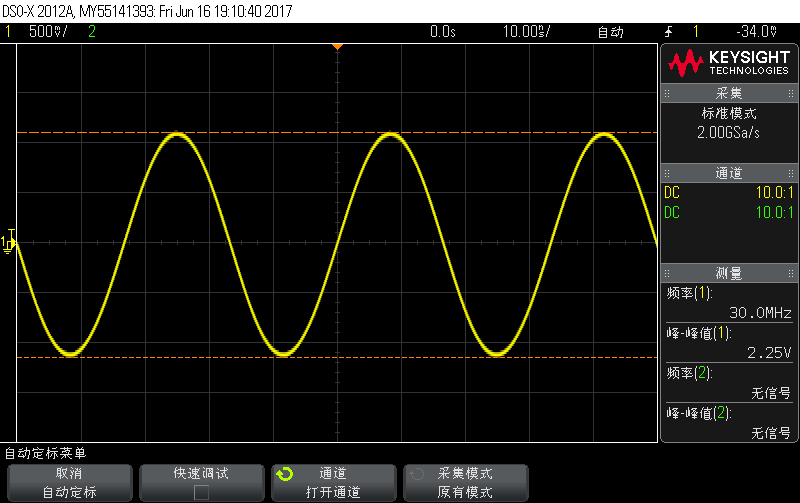
\includegraphics[width=0.7\linewidth]{imgs/scope_26.png}
	\caption{Origin voltage figure of $R=10\unit{k\Omega}$}
	\label{fig-1-1}
\end{figure}

When the temperature was raised, the comparison of the origin figure and the new figure was shown in Figure \ref{fig-1-2}.

\begin{figure}[htbp]
	\centering
	\subfigure[origin]{
		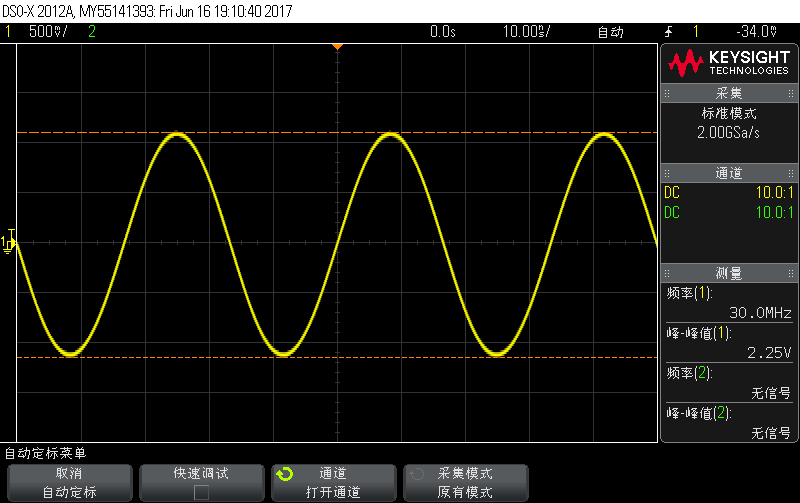
\includegraphics[width=0.45\linewidth]{imgs/scope_26.png}
		\label{fig-1-2-1}
	}
	\subfigure[higher temperature]{
		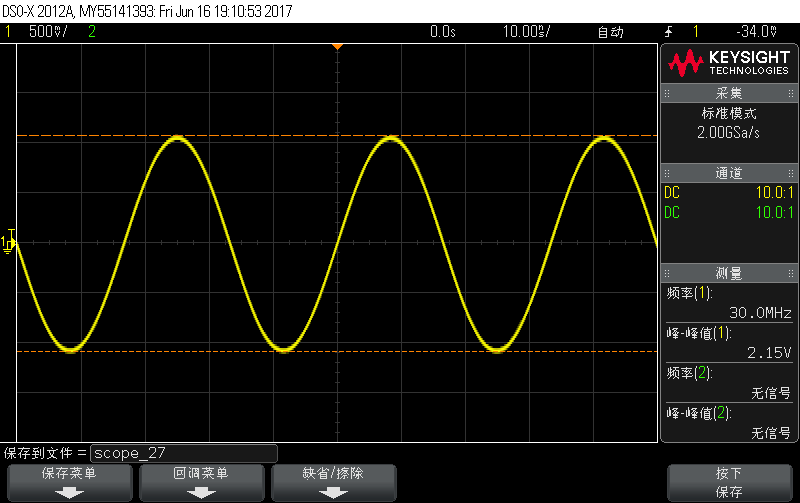
\includegraphics[width=0.45\linewidth]{imgs/scope_27.png}
		\label{fig-1-2-2}
	}
	\caption{Comparison between origin figure and higher temperature}
	\label{fig-1-2}
\end{figure}

We can find that when the temperature rises, the voltage on the source become slightly higher, which means that the resistance becomes higher.

\newpage
When the humidity was raised, the comparison of the origin figure and the new figure was shown in Figure \ref{fig-1-3}.

\begin{figure}[htbp]
	\centering
	\subfigure[origin]{
		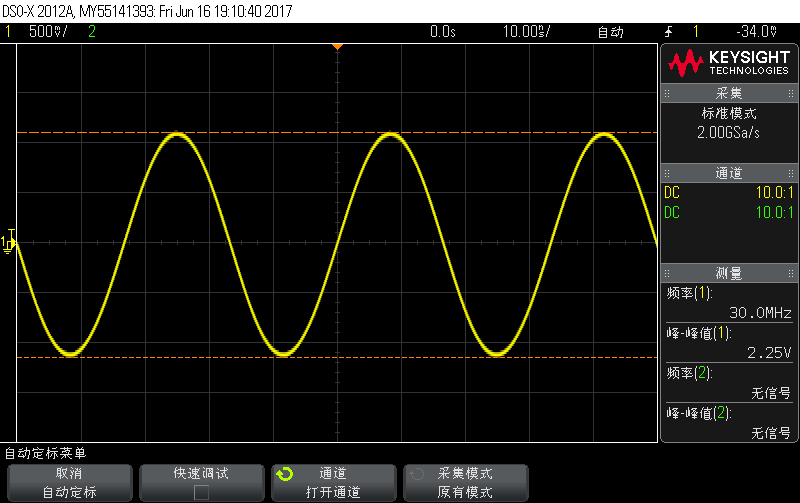
\includegraphics[width=0.45\linewidth]{imgs/scope_26.png}
		\label{fig-1-3-1}
	}
	\subfigure[higher humidity]{
		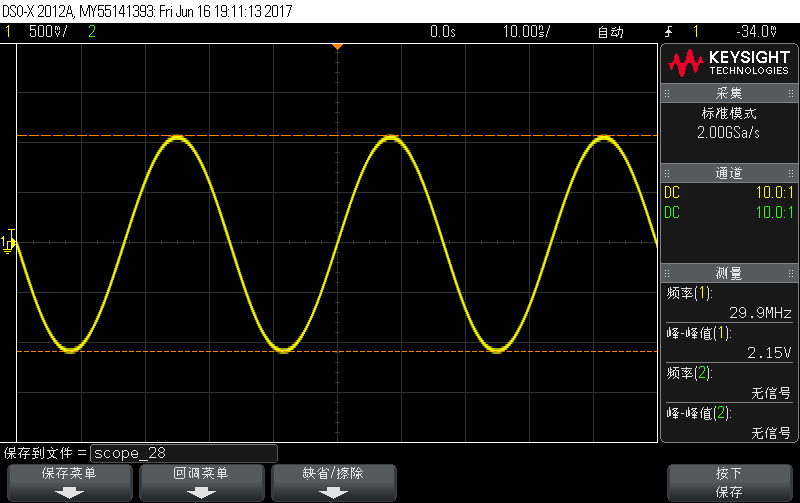
\includegraphics[width=0.45\linewidth]{imgs/scope_28.png}
		\label{fig-1-3-2}
	}
	\caption{Comparison between origin figure and higher humidity}
	\label{fig-1-3}
\end{figure}

We can find that when the humidity rises, the voltage on the source become slightly higher, which means that the resistance becomes higher.

\newpage

\subsection{Capacitors}

We choose two capacitors, 3.3$\unit{\mu F}$ and 0.082$\unit{\mu F}$.

For the 3.3$\unit{\mu F}$ capacitor, the figure was shown in Figure \ref{fig-2-1}.

\begin{figure}[htbp]
	\centering
	\subfigure[60 Hz]{
		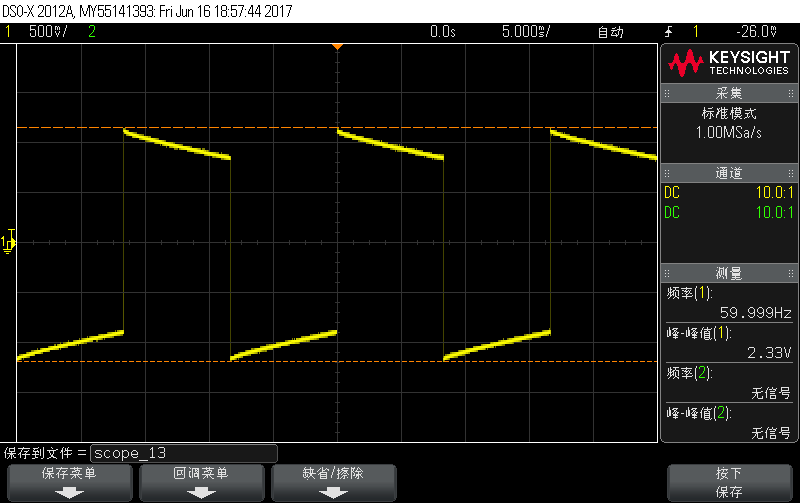
\includegraphics[width=0.45\linewidth]{imgs/scope_13.png}
		\label{fig-2-1-1}
	}
	\subfigure[10 kHz]{
		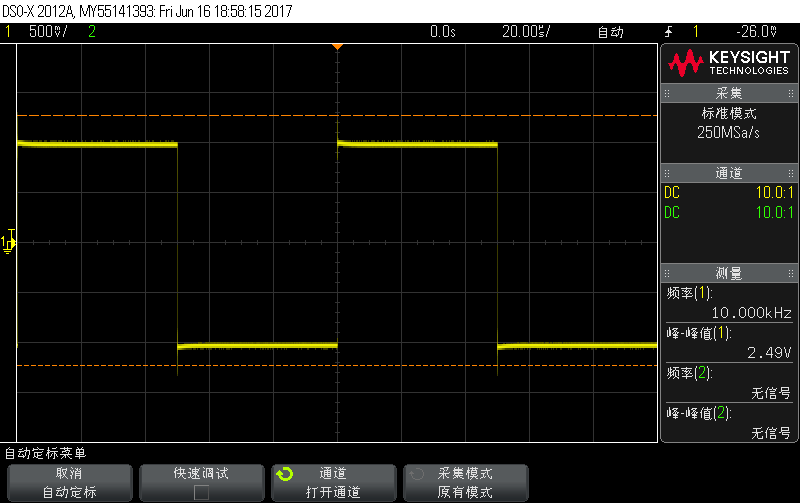
\includegraphics[width=0.45\linewidth]{imgs/scope_14.png}
		\label{fig-2-1-2}
	}
	\subfigure[1 MHz]{
		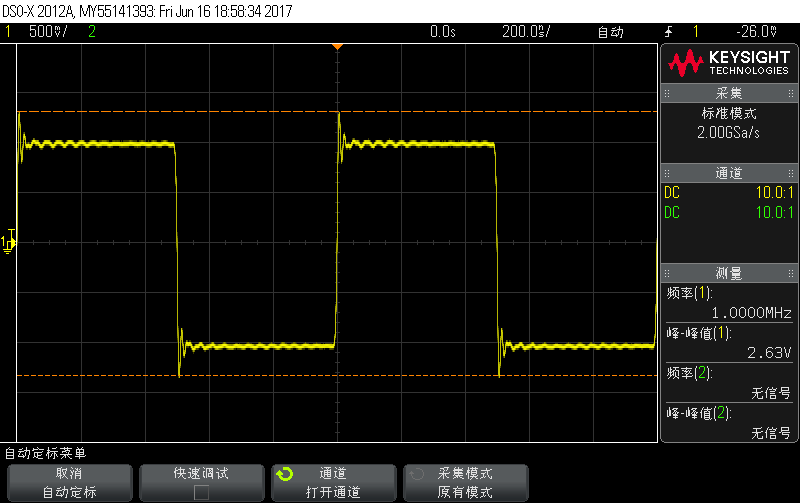
\includegraphics[width=0.45\linewidth]{imgs/scope_15.png}
		\label{fig-2-1-3}
	}
	\subfigure[10 MHz]{
		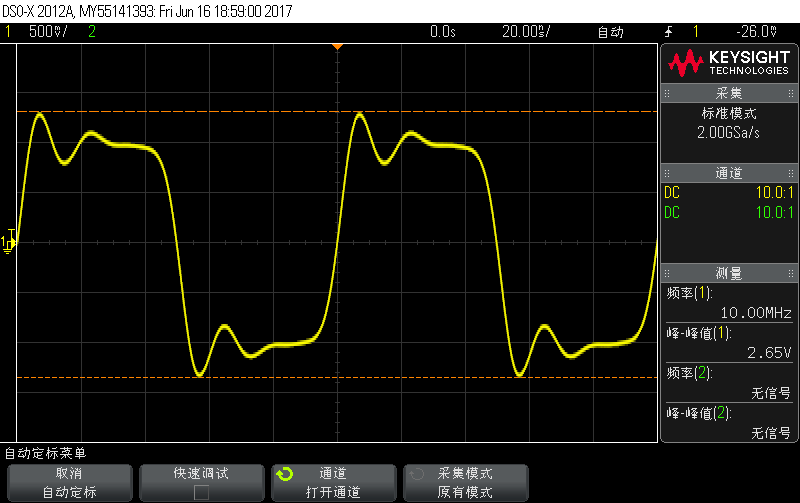
\includegraphics[width=0.45\linewidth]{imgs/scope_16.png}
		\label{fig-2-1-4}
	}
	\caption{3.3$\unit{\mu F}$ capacitor}
	\label{fig-2-1}
\end{figure}

\newpage

For the 0.082$\unit{\mu F}$ capacitor, the figure was shown in Figure \ref{fig-2-2}.

\begin{figure}[htbp]
	\centering
	\subfigure[60 Hz]{
		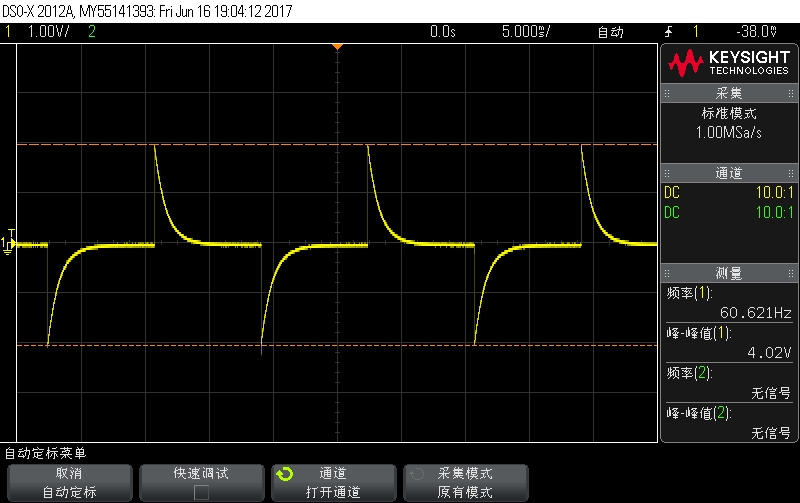
\includegraphics[width=0.45\linewidth]{imgs/scope_18.png}
		\label{fig-2-2-1}
	}
	\subfigure[10 kHz]{
		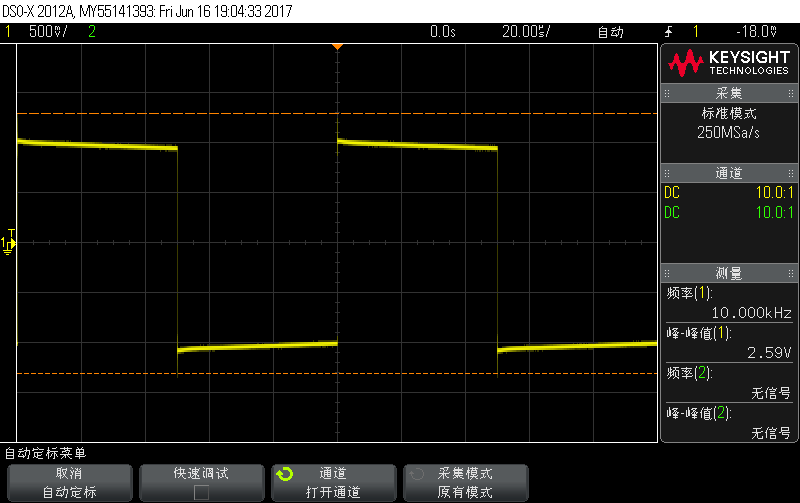
\includegraphics[width=0.45\linewidth]{imgs/scope_19.png}
		\label{fig-2-2-2}
	}
	\subfigure[1 MHz]{
		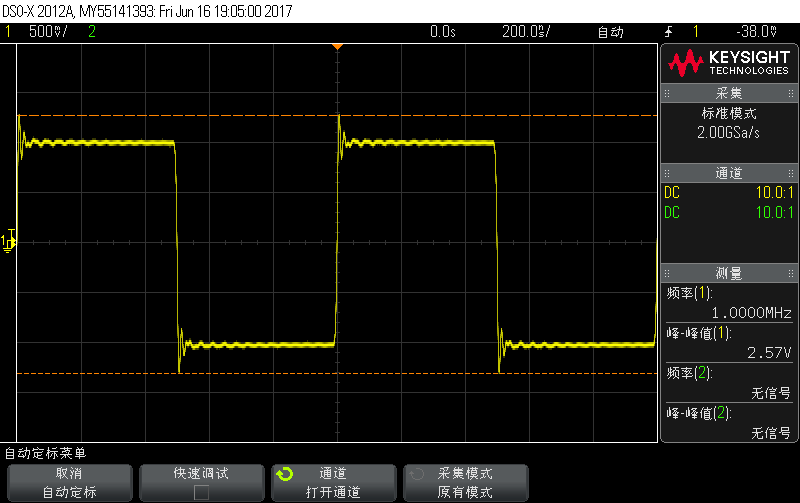
\includegraphics[width=0.45\linewidth]{imgs/scope_20.png}
		\label{fig-2-2-3}
	}
	\subfigure[10 MHz]{
		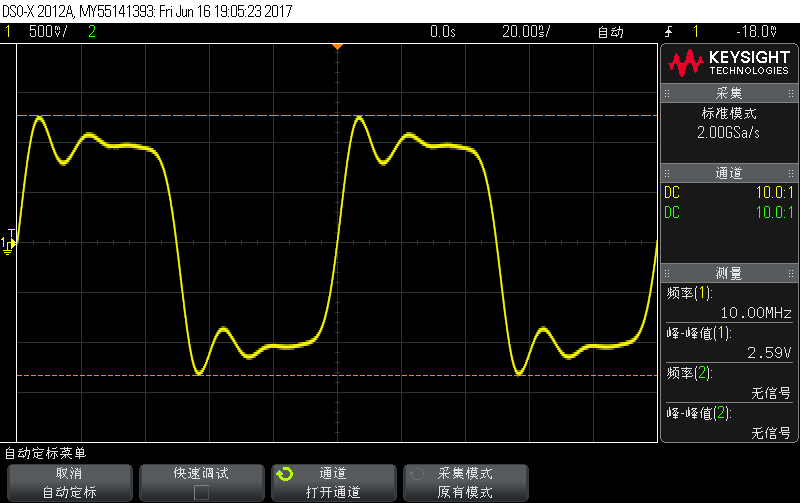
\includegraphics[width=0.45\linewidth]{imgs/scope_21.png}
		\label{fig-2-2-4}
	}
	\caption{0.082$\unit{\mu F}$ capacitor}
	\label{fig-2-2}
\end{figure}

\newpage
\subsection{Array of resistors}



\begin{figure}[htbp]
	\centering
	\subfigure[10 Hz]{
		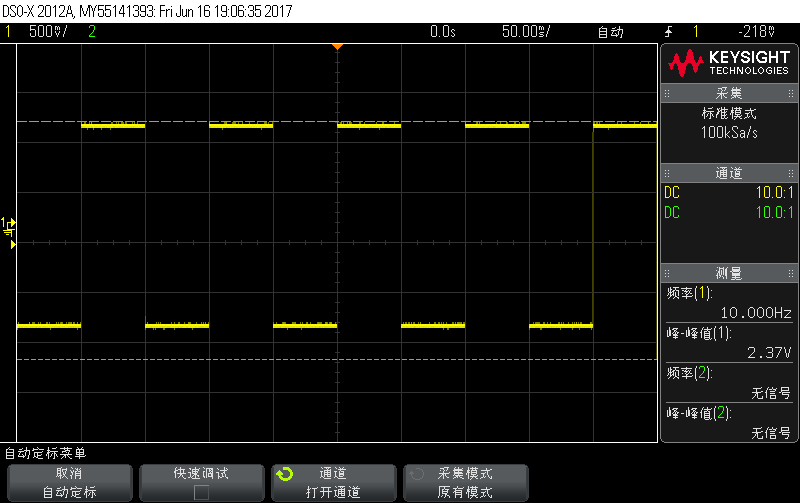
\includegraphics[width=0.45\linewidth]{imgs/scope_22.png}
		\label{fig-3-1}
	}
	\subfigure[10 kHz]{
		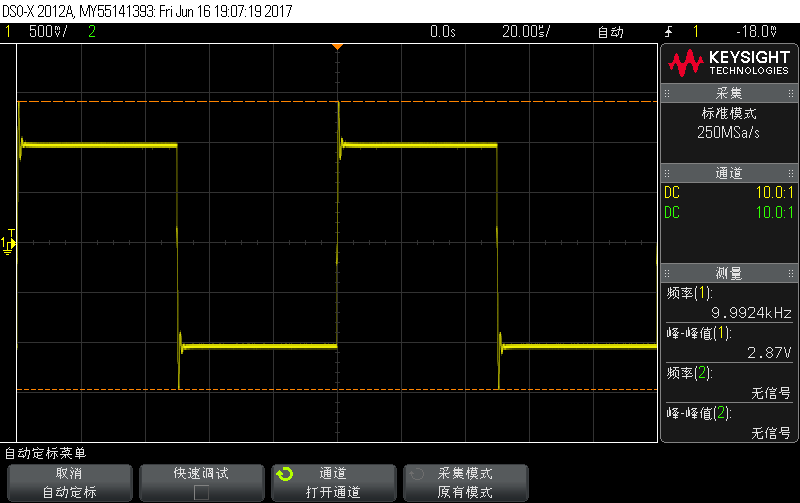
\includegraphics[width=0.45\linewidth]{imgs/scope_23.png}
		\label{fig-3-2}
	}
	\subfigure[10 MHz]{
		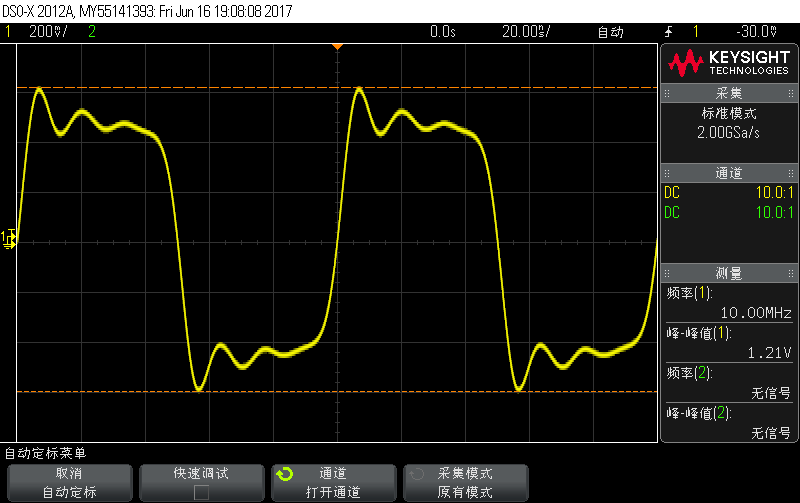
\includegraphics[width=0.45\linewidth]{imgs/scope_24.png}
		\label{fig-3-3}
	}
	\subfigure[30 MHz]{
		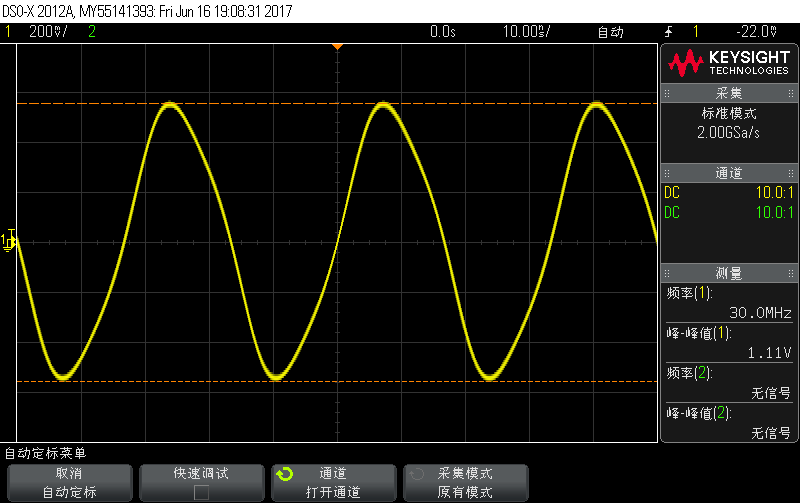
\includegraphics[width=0.45\linewidth]{imgs/scope_25.png}
		\label{fig-3-4}
	}
	\caption{0.082$\unit{\mu F}$ capacitor}
	\label{fig-3}
\end{figure}

\newpage
\section{Reference}

\subsection{References}
\begin{enumerate}
	\item Lab1 Manual
\end{enumerate}

\end{document}
